\documentclass[conference]{IEEEtran}
\IEEEoverridecommandlockouts
% The preceding line is only needed to identify funding in the first footnote. If that is unneeded, please comment it out.
\usepackage{cite}
\usepackage{amsmath,amssymb,amsfonts}
\usepackage{algorithmic}
\usepackage{graphicx}
\usepackage{textcomp}
\usepackage{xcolor}
\usepackage{tabularx}
\usepackage{multirow}
\usepackage{graphics} % for pdf, bitmapped graphics files
\usepackage{subfig}
\usepackage{subcaption}
\usepackage{hyperref}
\usepackage{academicons}
\usepackage{xcolor}
\usepackage{listings}
\usepackage{tabularx} % Asegúrate de incluir este paquete

\usepackage{tikz}
\usetikzlibrary{shapes.geometric, arrows}

\usetikzlibrary{shapes.geometric, arrows}

\tikzstyle{startstop} = [rectangle, rounded corners, minimum width=3cm, minimum height=1cm,text centered, draw=black, fill=red!30]
\tikzstyle{process} = [rectangle, minimum width=3cm, minimum height=1cm, text centered, draw=black, fill=blue!30]
\tikzstyle{arrow} = [thick,->,>=stealth]


\def\BibTeX{{\rm B\kern-.05em{\sc i\kern-.025em b}\kern-.08em
		T\kern-.1667em\lower.7ex\hbox{E}\kern-.125emX}}

% Color Enlace
\definecolor{colorEnlace}{RGB}{0, 0, 0}
\hypersetup{
	colorlinks=true,
	linkcolor=colorEnlace,
	citecolor=colorEnlace,
	urlcolor=colorEnlace,
	pdfauthor={Davis Bremdow Salazar Roa},
	pdftitle={Sistemas Embebidos}
}
\lstset{
	language=C,
	basicstyle=\ttfamily\small,
	keywordstyle=\color{blue},
	stringstyle=\color{red},
	commentstyle=\color{green!60!black},
	showstringspaces=false,
	numbers=left,
	numberstyle=\tiny\color{gray},
	frame=none,
	breaklines=true,
	tabsize=1
}

% Control 
\usepackage{amsmath}
\begin{document}
	
	\title{Informe final - Amplificador Diferencial Retroalimentado}
	\author{
		\makebox[\textwidth][c]{\large\textbf{Universidad Nacional de San Antonio Abad del Cusco}}\\
		\makebox[\textwidth][c]{\normalsize\textit{Escuela profesional de Ingeniería Electrónica}}\\
		\makebox[\textwidth][c]{\normalsize\textit{Laboratorio de Circuitos Electrónicos III}}\\
		\and
		\IEEEauthorblockN{Ing. Miguel Angel Janqui Cavero}
		\IEEEauthorblockA{Ingeniero Electrónico \\
			Cusco, Perú \\
			miguel.janqui@unsaac.edu.pe}
		\and
		\IEEEauthorblockN{Ruth Juana Espino Puma - 185746}
		\IEEEauthorblockA{Estudiante de Ingeniería Electrónica \\
			Cusco, Perú \\
			184657@unsaac.edu.pe}
		\and
		\IEEEauthorblockN{Davis Bremdow Salazar Roa - 200353}
		\IEEEauthorblockA{Estudiante de Ingeniería Electrónica \\
			Cusco, Perú \\
			200353@unsaac.edu.pe}
	}
	
	\maketitle
	\begin{abstract}
		Los circuitos resonantes son fundamentales en la recepción de señales de radiofrecuencia (RF) debido a su capacidad para seleccionar una frecuencia específica entre muchas presentes en el espectro electromagnético. Funcionan como filtros sintonizables que amplifican la señal deseada y atenúan las no deseadas, mejorando así la relación señal/ruido y la sensibilidad del receptor. Además, facilitan la demodulación eficiente al permitir que solo las señales de interés pasen a las siguientes etapas del sistema, como el mezclador o el amplificador. Su correcta implementación es clave para lograr una recepción clara y precisa en sistemas de comunicación inalámbrica.
	\end{abstract}
	\begin{IEEEkeywords}
		Resonancia, Selectividad, Frecuencia RF, Filtro Pasa Banda, Receptores RF, Sintonía, Amplificación, Demodulación
	\end{IEEEkeywords}
	
	\section{Curva teórica $I_O$ del circuito resonante en serie}
	
	En el primer circuito se realizo la simulación del mismo para la obtención de las características eléctricas destacando dentro de sus propiedades una máxima magnitud de corriente en la salida debido a la conexión de los elementos resistivos y reactivos en serie.
	
	Los valores de salida se obtuvieron e 2 formas
	\begin{itemize}
		\item Forma experimental mediante la simulación 
		\item De forma teórica
	\end{itemize}
	
	Siendo así que para el segundo método se hizo uso de la ecuación \ref{eq:corriente-serie} en la cual se obtiene la corriente de salida en función al voltaje de entrada y la magnitud de la impedancia total del circuito en resonancia.
	
	Además como se puede apreciar en \ref{eq:corriente-serie} el valor de corriente $I_O$ depende de la frecuencia, por lo que será necesario tabular y realizar este calculo para frecuencias por encima y por debajo de la frecuencias de resonancias $F_O$.
	
	\begin{equation}
		I_o = \frac{V_o}{Z} = \frac{V_o}{\sqrt{(R + R_1)^2 + (\omega L - \frac{1}{\omega C})^2}}
		\label{eq:corriente-serie}
	\end{equation}
	
	En la figura \ref{fig:circuito-serie} se puede apreciar el circuito simulado con los valores de resistencias y reactancia asignados en la guía en el cual se configuraron dos multímetros configurados para una medición de señal alterna para medir el voltaje de salida y la corriente para cada valor de frecuencia.
	
	\begin{figure}[h]
		\centering
		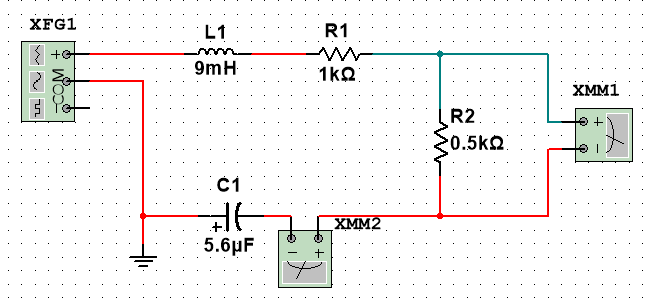
\includegraphics[width=0.4\textwidth]{circuito-serie}
		\caption{Circuito Resonante en Serie}
		\label{fig:circuito-serie}
	\end{figure}
	
	Además de ello también se agrego un osciloscopio en la salida para determinar la forma de onda y el desfase de la señal de salida para valores muy por debajo y encima de la frecuencia de resonancia, siendo así que el resumen de valores medidos para el circuito serie se muestra en la tabla \ref{tab:mediciones-serie}.
	
	\begin{table}[h]
		\centering
		\begin{tabular}{|ccc|}
			\hline
			\multicolumn{3}{|c|}{\textbf{Barrido   de frecuencias}}                                                  \\ \hline
			\multicolumn{1}{|c|}{\textbf{f (Hz)}} & \multicolumn{1}{c|}{\textbf{Vo {[}mV{]}}} & \textbf{Io {[}mA{]}} \\ \hline
			\multicolumn{1}{|c|}{10}              & \multicolumn{1}{c|}{333.437}              & 0.666875             \\ \hline
			\multicolumn{1}{|c|}{20}              & \multicolumn{1}{c|}{516.629}              & 1.033                \\ \hline
			\multicolumn{1}{|c|}{50}              & \multicolumn{1}{c|}{662.684}              & 1.325                \\ \hline
			\multicolumn{1}{|c|}{100}             & \multicolumn{1}{c|}{695.498}              & 1.391                \\ \hline
			\multicolumn{1}{|c|}{200}             & \multicolumn{1}{c|}{704.455}              & 1.409                \\ \hline
			\multicolumn{1}{|c|}{300}             & \multicolumn{1}{c|}{706.099}              & 1.412                \\ \hline
			\multicolumn{1}{|c|}{400}             & \multicolumn{1}{c|}{706.733}              & 1.413                \\ \hline
			\multicolumn{1}{|c|}{500}             & \multicolumn{1}{c|}{706.954}              & 1.414                \\ \hline
			\multicolumn{1}{|c|}{600}             & \multicolumn{1}{c|}{707.086}              & 1.414                \\ \hline
			\multicolumn{1}{|c|}{700}             & \multicolumn{1}{c|}{707.1}                & 1.414                \\ \hline
			\multicolumn{1}{|c|}{708.93}          & \multicolumn{1}{c|}{707.1}                & 1.414                \\ \hline
			\multicolumn{1}{|c|}{850}             & \multicolumn{1}{c|}{707.063}              & 1.414                \\ \hline
			\multicolumn{1}{|c|}{950}             & \multicolumn{1}{c|}{706.984}              & 1.414                \\ \hline
			\multicolumn{1}{|c|}{1000}            & \multicolumn{1}{c|}{706.939}              & 1.414                \\ \hline
			\multicolumn{1}{|c|}{1200}            & \multicolumn{1}{c|}{706.757}              & 1.414                \\ \hline
			\multicolumn{1}{|c|}{2000}            & \multicolumn{1}{c|}{705.517}              & 1.411                \\ \hline
			\multicolumn{1}{|c|}{2500}            & \multicolumn{1}{c|}{704.37}               & 1.409                \\ \hline
			\multicolumn{1}{|c|}{3500}            & \multicolumn{1}{c|}{701.313}              & 1.403                \\ \hline
			\multicolumn{1}{|c|}{5000}            & \multicolumn{1}{c|}{695.028}              & 1.39                 \\ \hline
		\end{tabular}
		\caption{Valores simulados experimentalmente - Circuito Serie}
		\label{tab:mediciones-serie}
	\end{table}
		
	
	
	
	
	Mostrándose la evolución de la corriente de forma gráfica para el método experimental en la figura \ref{fig:grafica-corriente-serie}
	
	\begin{figure}[h]
		\centering
		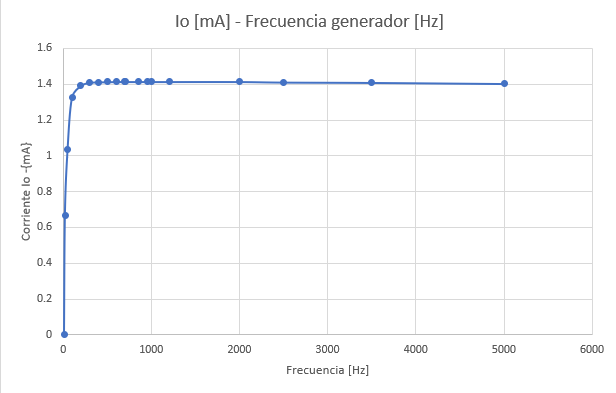
\includegraphics[width=0.5\textwidth]{grafica-corriente-serie}
		\caption{Corriente en función de la frecuencia - Circuito Serie}
		\label{fig:grafica-corriente-serie}
	\end{figure}
	

	\section{Curva teórica $I_O$ del circuito resonante en paralelo}
	\begin{equation}
		I_o = \frac{V_o}{Z} = \frac{V_o}{\sqrt{R^2 + \frac{\omega^2 L^2}{(1 - \omega^2 CL)^2}}}
		\label{eq:corriente-paralelo}
	\end{equation}

	% Contenido del documento
	
	\section{Curva real vs curva teórica}
	
	
	\bibliographystyle{IEEEtran}
	\bibliography{biblio}
\end{document}